\documentclass[tikz, border=6pt]{standalone}

\usepackage[T1]{fontenc}
\usepackage{helvet}
\renewcommand{\familydefault}{\sfdefault}

\usetikzlibrary{shapes.geometric, arrows.meta}

\tikzset{
    question/.style = {draw, rectangle, thick, align=center, inner sep=6pt, minimum height=1.2cm},
    exit/.style = {draw, ellipse, thick, align=center, inner sep=2pt, minimum height=1.5cm},
    branch/.style = {-{Latex[length=2.5mm]}, thick},
    answer/.style = {font=\small, inner sep=3pt},
}

\begin{document}

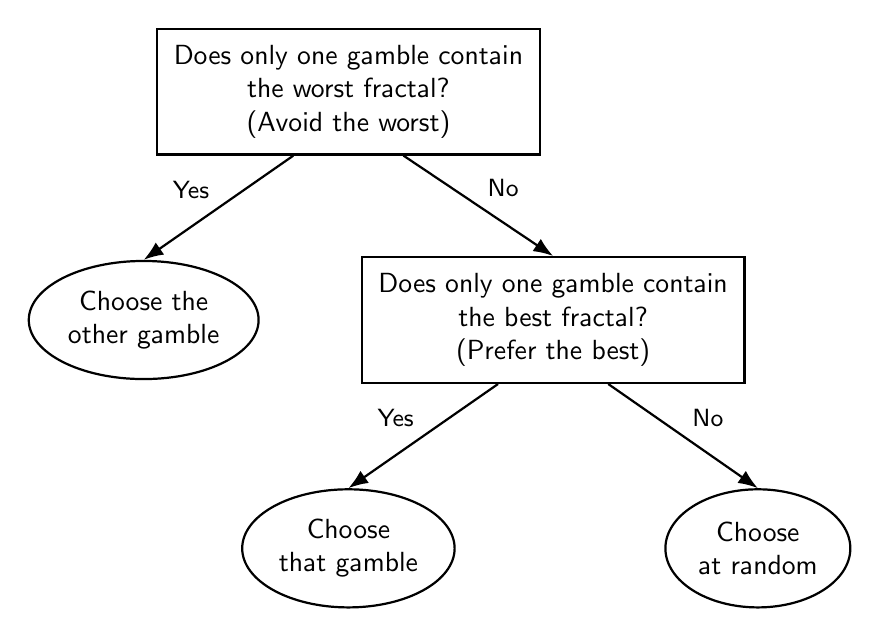
\begin{tikzpicture}[x = 2.6cm, y = 2.9cm]

  \node[question] (cue_avoid_worst) at (0, 0) {Does only one gamble contain\\the worst fractal?\\(Avoid the worst)};

  \node[exit]     (exit_avoid_worst) at (-1, -1) {Choose the\\other gamble};
  \node[question] (cue_prefer_best)  at ( 1, -1) {Does only one gamble contain\\the best fractal?\\(Prefer the best)};

  \node[exit] (exit_prefer_best) at (0, -2) {Choose\\that gamble};
  \node[exit] (exit_random)      at (2, -2) {Choose\\at random};

  \draw[branch] ([xshift=-7mm]cue_avoid_worst.south) -- node[answer, above left]  {Yes} (exit_avoid_worst.north);
  \draw[branch] ([xshift= 7mm]cue_avoid_worst.south) -- node[answer, above right] {No}  (cue_prefer_best.north);

  \draw[branch] ([xshift=-7mm]cue_prefer_best.south) -- node[answer, above left]  {Yes} (exit_prefer_best.north);
  \draw[branch] ([xshift= 7mm]cue_prefer_best.south) -- node[answer, above right] {No}  (exit_random.north);

\end{tikzpicture}

\end{document}
